\documentclass{ML}
\usepackage{fontspec}
\usepackage{color}
\usepackage{multicol}
\newminted{text}{framesep=2mm,fontsize=\scriptsize, linenos}
\newminted{python}{frame=lines, framesep=2mm, linenos}
\newminted{c}{frame=lines, framesep=2mm, linenos}
\newminted{java}{frame=lines, framesep=2mm, linenos}
\newfontfamily\unicodefont{Courier New}
% 姓名,学号
\infoauthor{朱明彦}{1160300314}

% 课程类型,实验名称
\infoexp{课程类型}{大作业}

\infoschool{计算机学院}{辛明影}

\begin{document}
\maketitle

\tableofcontents
\newpage

\begin{center}
    \textbf{\zihao{3} 编译原理 大作业}
\end{center}

\section{需求分析}
在词法分析、语法分析和语义分析的实验基础之上,结合代码优化等技术,将之前的\texttt{Lexer, Parser}结合起来,形成一个完整的编译器前端程序。
\section{关键字定义与文法设计}
\subsection{关键字定义}
在词法分析部分对于关键字的定义是通过\texttt{Java}中的枚举类型来实现。
\begin{javacode}
public enum Tag {
    INT("int"), FLOAT("float"), BOOL("bool"), CHAR("char"), RECORD("record"), 
    IF("if"), ELSE("else"), DO("do"), WHILE("while"), 
    BREAK("break"), CONTINUE("continue"), TRUE("true"), 
    FALSE("false"), RETURN("return"),// keyword
    
    ADD("+"), SUB("-"), MUL("*"), DIV("/"), MOD("%"), // arithmetic op

    NE("!="), G(">"), GE(">="), L("<"), LE("<="), EQ("=="), 
    AND("&&"), OR("||"), NOT("!"), // logical op
    
    SLP("("), SRP(")"), LP("{"), RP("}"), MLP("["), MRP("]"), 
    ASSIGN("="), SEMICOLON(";"), COMMA(","), // delimiters
    
    REAL("real"), // float number
    NUM("num"), // integer number
    ID("id"),  // identifier
    STRING("string"),
    STACK_BOTTOM(Parser.STACK_BOTTOM_CHARACTER),
    PROC("proc"), CALL("call"),
    NULL("null");
// 仅列出关键字部分 其余详见src/lexer/Tag.java
}
\end{javacode}
\subsection{文法设计}\label{sec:grammar}
最终实现的文法以及语义动作的定义如下所示,其中{\color{red}红色}字体为该产生式对应的语义动作。
\begin{enumerate}
    {\unicodefont \footnotesize
    \item Start -> P 
    \vspace{0.5cm}
    
    \item P -> PStart D P \textbf{|}
    
    \hspace{1cm}PStart S P \textbf{|} $\epsilon$
    
    \vspace{0.5cm}
    
    \item PStart -> $\epsilon$ {\color{red}\{ env = new Env(env); offsetStack.push(offset); offset=0;\}}
    \vspace{0.5cm}
    
    \item D -> proc X id ( M ) DM { P } {\color{red}\{pop(tableStack); pop(offset)\}} \textbf{|}
    
    \hspace{1cm} record id { P } \textbf{|}
    
    \hspace{1cm} T id A ; {\color{red}\{enter(id.lexeme, T.type, offset);offset = offset + T.width;\}}
        \vspace{0.5cm}
    
    \item DM -> $\epsilon$ {\color{red}\{table = mkTable(top(tableStack)); push(table); push(offset); offset = 0;\}}
    \vspace{0.1cm}
    
    \item A -> = F A \textbf{|} , id A \textbf{|} $\epsilon$
    \vspace{0.5cm}
    
    \item M -> M , X id {\color{red}\{enter(id.lexeme, X.type, offset); offset = offset + X.width; M.size = M1.size + 1;\}} \textbf{|} 
    
    \hspace{0.5cm}X id {\color{red}\{enter(id.lexeme, X.type, offset); offset = offset + X.width; M.size = 1;\}}
    \vspace{0.1cm}
    
    \item T -> X {\color{red}\{t = X.type; w = X.width;\}} C {\color{red}\{T.type = C.type; T.width = C.width;\}}
    \vspace{0.5cm}
    
    \item X -> int {\color{red}\{X.type = interger; X.width = 4;\}}\textbf{|} 
    
    \hspace{1cm}float {\color{red}\{X.type = float; X.width = 8;\}} \textbf{|}
         bool \textbf{|} char
    \vspace{0.5cm}
    
    \item C -> [ num ] C {\color{red}\{C.type = C1.type + '[' + num.value + ']'; C.width = num.value * C1.width;\}} \textbf{|}
         $\epsilon$ {\color{red}\{C.type = t; C.width = w;\}}
    
         \vspace{0.5cm}
    \item S -> id = E ; {\color{red}\{S.nextList = null; p = loopUp(id.lexeme); if p == null then error else gen(p, '=', E.addr);\}} \textbf{|}
    
    \hspace{1cm}if ( B ) BM S N else BM S {\color{red}\{backpatch(B.trueList, BM1.instr); backpatch(B.falseList, BM2.instr); temp = merge(S1.nextList, N.nextList); S.nextList = merge(temp, S2.nextList); \}} \textbf{|} 
    
    \hspace{1cm}while BM ( B ) BM S {\color{red}\{backpatch(S1.nextList, BM1.instr); backpatch(B.trueList, BM2.instr); S.nextList = B.falseList; gen('goto', BM1.instr); \}} \textbf{|} 
    
    \hspace{1cm}call id ( Elist ) ; \textbf{|} return E ; \textbf{|} if ( B ) BM S {\color{red}\{backpatch(B.trueList, BM.instr); S.nextList = merge(B.falseList, S1.nextList); \}} \textbf{|} 
    
    \hspace{1cm}L = E ; {\color{red}\{gen(L.array, L.addr, '=', E.addr)\}}
    \vspace{0.5cm}
    
    \item N -> $\epsilon$ {\color{red}\{N.nextList = makeList(nextInstr); gen('goto'); \}}
    
    \vspace{0.5cm}
    \item L -> L [ E ] {\color{red}\{L.array = L1.array; L.type = L1.type.elem; L.width = L.type.width; t = new Temp(); L.addr = new Temp(); gen(L.addr, '=', E.addr, '*', L.width); gen(L.addr, '=', L1.addr, '+', t); \}} \textbf{|} 
    
    \hspace{1cm}id [ E ] {\color{red}\{p = lookUp(id.lexeme); if p == null then error else L.array = p; L.type = id.type; L.addr = new Temp(); gen(L.addr, 'addr', E.addr, '*', L.width)\}}
    \vspace{0.5cm}
    
    \item E -> E + G {\color{red}\{E.addr = newTemp(); gen(E.addr, '=', E1.addr, '+', G.addr);\}} \textbf{|}
    
    \hspace{1cm}G {\color{red}\{E.addr = G.addr;\}}
    
    \vspace{0.5cm}
    \item G -> G * F {\color{red}\{G.addr = newTemp(); gen(G.addr, '=', G1.addr, '*', F.addr);\}}\textbf{|} 
    
    \hspace{1cm}F {\color{red}\{G.addr = F.addr;\}}
    \vspace{0.5cm}
    
    \item F -> ( E ) {\color{red}\{F.addr = E.addr;\}} \textbf{|} 
    
    \hspace{1cm}num {\color{red}\{F.addr = num.value;\}} \textbf{|}
    
    \hspace{1cm}id {\color{red}\{F.addr = lookup(id.lexeme); if F.addr == null then error;\}}\textbf{|} real {\color{red}\{F.addr = real.value;\}}\textbf{|} string \textbf{|} L {\color{red}\{F.addr = L.array + '[' + L.addr']'\}}
    \vspace{0.5cm}
    
    \item B -> B || BM H {\color{red}\{backpatch(B1.falseList, BM.instr); B.trueList = merge(B1.trueList, H.trueList); B.falstList = H.falstList;\}} \textbf{|}
    
    \hspace{1cm}H {\color{red}\{B.trueList = H.trueList; B.falseList = H.falseList;\}}
    \vspace{0.5cm}
    
    \item H -> H \&\& BM I {\color{red}\{backpatch(H1.trueList, BM.instr); H.trueList = I.trueList; H.falseList = merge(H1.falseList, I.falseList);\}} \textbf{|}
    
    \hspace{1cm}I {\color{red}\{H.trueList = I.trueList; H.falseList = I.falseList;\}}
    \vspace{0.5cm}
    
    \item I -> ! I {\color{red}\{I.trueList = I1.falseList; I.falseList = I1.falseList;\}} \textbf{|}
    
    \hspace{1cm}( B ) {\color{red}\{I.trueList = B.trueList; I.falseList = B.falseList;\}} \textbf{|}
    
    \hspace{1cm}E Relop E {\color{red}\{I.trueList = makeList(nextInstr); I.falseList = makeList(nextInstr + 1); gen('if', E1.addr, Relop.op, E2.addr, 'goto'); gen('goto');\}} \textbf{|}
    
    \hspace{1cm}true {\color{red}\{I.trueList = makeList(nextInstr); gen('goto');\}} \textbf{|}
    
    \hspace{1cm}false {\color{red}\{I.falseList = makeList(nextInstr); gen('goto');\}}
    \vspace{0.5cm}
    
    \item BM -> $\epsilon$ {\color{red}\{BM.instr = nextInstr\}}
    \vspace{0.5cm}
    
    \item Relop -> < \textbf{|} <= \textbf{|} > \textbf{|} >= \textbf{|} == \textbf{|} != {\color{red}\{Relop.op = op\}}
    \vspace{0.5cm}
    
    \item Elist -> Elist , E {\color{red}\{Elist.size = Elist1.size + 1;\}} \textbf{|}
         E {\color{red}\{Elist.size = 1;\}}
    }
\end{enumerate}

\textbf{为了语义动作的设计,以上文法为二义文法,在\texttt{Parser}中设计为移进优先于规约,解决了\texttt{else悬空}的问题,具体见\texttt{src/parser/Parser.java}}。
\section{系统设计}
\subsection{编译器框架}
\begin{figure}[H]
    \centering
    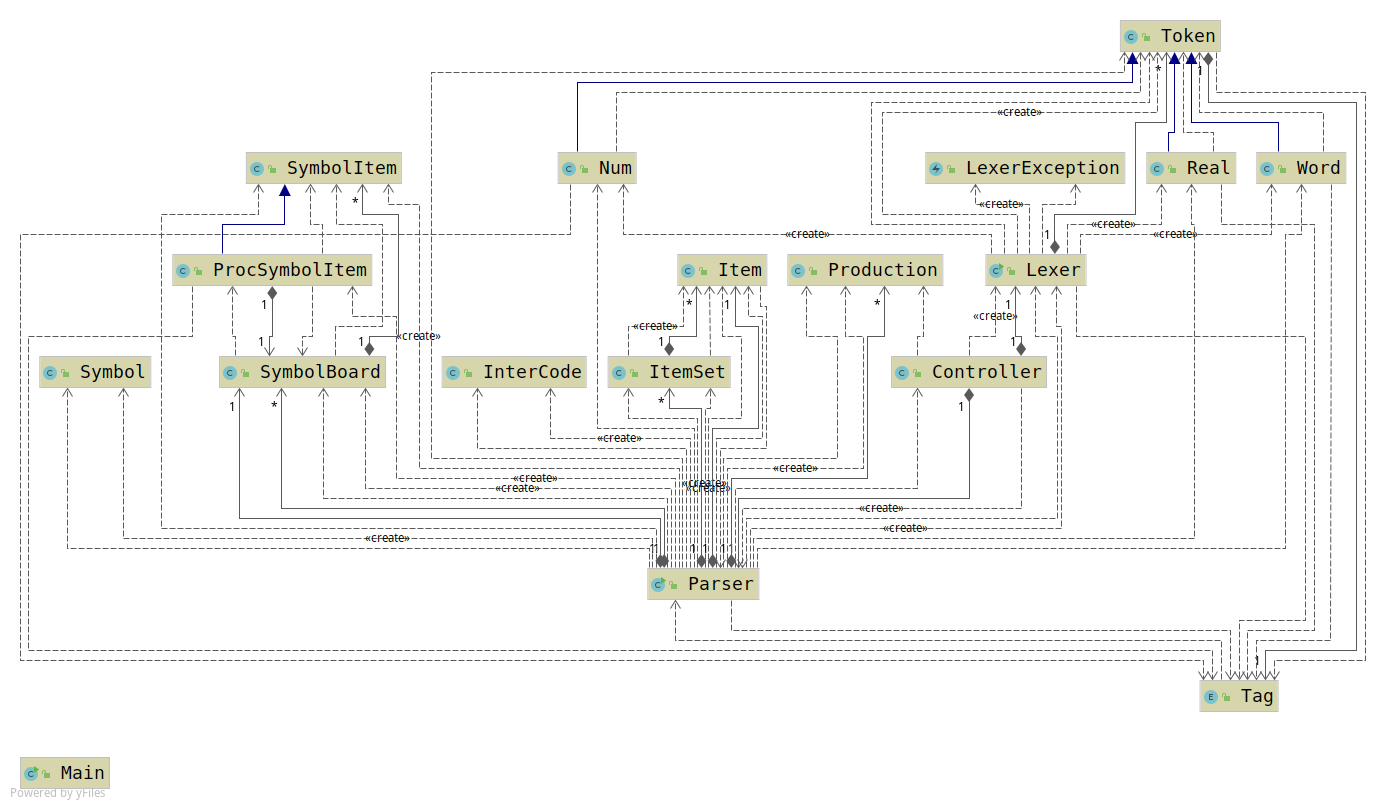
\includegraphics[width=1\linewidth]{media/Compiler.png}
    \caption{编译器框架图}\label{fig:compiler}
\end{figure}

对于大作业最终实现的编译器,其UML图如\ref{fig:compiler}所示,下面分别对其中不同的实现进行阐述。
\begin{itemize}
    \item \texttt{Lexer}为整个编译器的词法分析器部分,其可以将输入的类C语言源文件转化为Token序列,并作为下一步语法分析器的输入。
    \item \texttt{Parser}为整个编译器的语法分析器部分,在本项目中实现了LR(1)分析法,并在语法分析的同时进行语义动作,即所有的语义动作作用的属性均为S属性\cite{dragon-book},最终结果为中间代码。
    \item \texttt{Controller}为整个编译器GUI的控制部分,其使用\texttt{JavaFX}实现。
    \item \texttt{Main}为整个编译器的主程序部分,启动GUI形式的编译器,调用\texttt{Main}对应的主函数即可。
    \item \texttt{Token, Real, Num, Word}分别为\texttt{Lexer}输出的Token的父类、浮点型常数类、整数常数类以及标识符和字符串型常数类的父类。
    \item \texttt{Tag}为标注Token类别的枚举类型。
    \item \texttt{LexerException}为发现词法分析错误抛出的异常类。
    \item \texttt{Production}为语法中的产生式类,分别记录产生式左部和右部。
    \item \texttt{Item, ItemSet}分别为项目类和项目集类,其中项目类即在进行LR(1)语法分析时,对应的“项目”概念的类,即文法中的一个产生式和位于它的右部中某处的点组成;项目集类,则是项目的集合。
    \item \texttt{InterCode}为\texttt{Parser}最终结果对应的中间代码类。
    \item \texttt{SymbolItem, ProcSymbolItem}分别对应符号表中表项的父类和符号表中方法表项类,其区别为方法表项中包含其对应的局部符号表。
    \item \texttt{SymbolBoard}为符号表类,其包含的表项均为\texttt{SymbolItem}类。
    \item \texttt{Symbol}为产生式中的符号类,或者称为非终结符类,其在产生式中的右部时可能会包含S属性,方便语义分析时的语义动作处理。
\end{itemize}

\subsection{核心数据结构}
在本项目的所实现的编译器中,所用的数据结构有\texttt{栈、队列、集合、Map和多维数组},其中\texttt{栈}为最重要的数据结构。
下面分别阐述各个数据结构在编译器中起到的作用。

\begin{itemize}
    \item \textbf{栈(Stack)},作为核心数据结构,在\texttt{Parser}中使用栈记录调用关系,包括记录offset和符号表。
    \item \textbf{队列(Queue)},在\texttt{Lexer}中作为输入缓冲实现,其作用是进行一些有二义符号,如$>, >=$。
    \item \textbf{集合(Set)},其多次出现在本项目的实现中,分别作为\texttt{Lexer}中各种符号的记录,\texttt{Parser}中产生式、终结符、非终结符以及项目集族的记录。
    \item \textbf{Map},其多次出现在本项目实现的Compiler中,如记录标识符与其对应的符号表条目、LR(1)分析法中记录非终结符的First集以及每个项目闭包的GOTO表。
    \item \textbf{Array},主要用于记录LR(1)分析表。
\end{itemize}

\subsection{主要函数功能}

\subsubsection{\texttt{Lexer}主要函数功能}

\begin{minted}{java}
    public void scan();
\end{minted}

对于\texttt{Lexer}中的\texttt{scan}函数而言,主要功能为将输入的源文件转化为对应的Token序列,负责完成\texttt{Lexer}的主要逻辑。

\subsubsection{\texttt{Parser}主要函数功能}
\begin{enumerate}
    
    \item \begin{minted}{java}
    public List<Production> reduce(List<Token> tokens);
    \end{minted}
    
    对于\texttt{Parser}中的\texttt{reduce}函数而言,由于在进行语法分析的同时可以进行语义分析,所以\texttt{reduce}函数完成了从词法分析器的Token序列,到语法分析的产生式序列的转换。
    并且在函数返回之前,将最终的中间代码进行代码优化并输出。

    \item \begin{minted}{java}
    public void items();
    \end{minted}

    在\texttt{Parser}中另一个核心函数就是\texttt{items},其实现的参考算法见\cite{dragon-book}在LR(1)分析法中提到的\textit{items()}算法,
    主要实现了解析语法文件并生成对应的LR分析表的过程。
\end{enumerate}
% \subsection{核心流程图}
% % TODO 

\section{系统实现}
    以下内容主要介绍在本项目中实现的Compiler里,用于测试完成情况的文件,以及中间结果的展示。
\subsection{源文件}\label{sec:source}
\begin{ccode}
    int a;
    a = 1 + 2;
    int b;
    int c;
    c = 10;
    b = c + 1;
    int d;
    d = c * 2;
    int e;
    e = 0;
    int x;
    int y;
    y = 999;
    int z;
    z = 100;
    while (a < b)
        if (c < d) x = y + z; else x = a + b;
    
    a = b + c * (d + e);
    
    if(a > b)
        c = d;
    
    proc float function(float i){
        i = i + 1;
        return i;
    }
        
        int [2][3] list;
        int c;
        int i;
        int j;
        int d;
        float h;
        d = c + list[i][j];
        list[i][j] = c;
        
        d = h * c;
        
        c[1][2] = d;
        proc int function(int a, int c){
            a = c + 10;
            int d;
            return a;
    }        
\end{ccode}

在以上的源文件中有\textit{变量的声明(包括普通变量和多维数组变量),变量的使用,分支结构(if-else),循环结构(while)以及函数的声明(使用proc关键字)}
等不同的语句。
\subsection{语法分析表}
\begin{table}[H]
    \centering
    \begin{tabular}{|l|l|l|l|l|l|l|l|}
    \hline
        & \&\&                    & ||                      & \textless{}=            & ... & A & B   & ... \\ \hline
    0   &                         &                         &                         &     &   &     &     \\ \hline
    1   &                         &                         &                         &     &   &     &     \\ \hline
    2   &                         &                         &                         &     &   &     &     \\ \hline
    3   &                         &                         &                         &     &   &     &     \\ \hline
    ... &                         &                         &                         &     &   &     &     \\ \hline
    58  &                         &                         &                         &     &   & 111 &     \\ \hline
    59  &                         &                         & r(F -\textgreater real) &     &   &     &     \\ \hline
    60  & r(I -\textgreater true) & r(I -\textgreater true) &                         &     &   &     &     \\ \hline
    61  &                         & s160                    &                         &     &   &     &     \\ \hline
    ... &                         &                         &                         &     &   &     &     \\ \hline
    398 &                         &                         &                         &     &   &     &     \\ \hline
    \end{tabular}
    \caption{LR分析表(部分)}\label{tab:lr}
\end{table}
经过\texttt{Parser}的\texttt{items}函数处理在第\ref{sec:grammar}节中定义的文法,经过LR(1)分析得到的分析表如表\ref{tab:lr}所示。
表\ref{tab:lr}中仅仅展示了部分LR分析表的内容,共有398个状态,对于终结符如左侧的$\&\&$,其对应的状态可能有移进如\texttt{s160}和规约如\texttt{r(I->true)}动作;
对于非终结符如右侧的\texttt{A,B}等,其表示在相应状态和栈顶符号时应该转移的状态,即\texttt{GOTO表}。

\textbf{完整的LR(1)分析表见\texttt{src/parser/LRTable.txt}所示}。
\subsection{Token序列}\label{sec:token}
\begin{multicols}{4}
\begin{textcode}
<INT>
<ID, a>
<SEMICOLON>
<ID, a>
<ASSIGN>
<NUM, 1>
<ADD>
<NUM, 2>
<SEMICOLON>
<INT>
<ID, b>
<SEMICOLON>
<INT>
<ID, c>
<SEMICOLON>
<ID, c>
<ASSIGN>
<NUM, 10>
<SEMICOLON>
<ID, b>
<ASSIGN>
<ID, c>
<ADD>
<NUM, 1>
<SEMICOLON>
<INT>
<ID, d>
<SEMICOLON>
<ID, d>
<ASSIGN>
<ID, c>
<MUL>
<NUM, 2>
<SEMICOLON>
<INT>
<ID, e>
<SEMICOLON>
<ID, e>
<ASSIGN>
<NUM, 0>
<SEMICOLON>
<INT>
<ID, x>
<SEMICOLON>
<INT>
<ID, y>
<SEMICOLON>
<ID, y>
<ASSIGN>
<NUM, 999>
<SEMICOLON>
<INT>
<ID, z>
<SEMICOLON>
<ID, z>
<ASSIGN>
<NUM, 100>
<SEMICOLON>
<WHILE>
<SLP>
<ID, a>
<L>
<ID, b>
<SRP>
<IF>
<SLP>
<ID, c>
<L>
<ID, d>
<SRP>
<ID, x>
<ASSIGN>
<ID, y>
<ADD>
<ID, z>
<SEMICOLON>
<ELSE>
<ID, x>
<ASSIGN>
<ID, a>
<ADD>
<ID, b>
<SEMICOLON>
<ID, a>
<ASSIGN>
<ID, b>
<ADD>
<ID, c>
<MUL>
<SLP>
<ID, d>
<ADD>
<ID, e>
<SRP>
<SEMICOLON>
<IF>
<SLP>
<ID, a>
<G>
<ID, b>
<SRP>
<ID, c>
<ASSIGN>
<ID, d>
<SEMICOLON>
<PROC>
<FLOAT>
<ID, function>
<SLP>
<FLOAT>
<ID, i>
<SRP>
<LP>
<ID, i>
<ASSIGN>
<ID, i>
<ADD>
<NUM, 1>
<SEMICOLON>
<RETURN>
<ID, i>
<SEMICOLON>
<RP>
<INT>
<MLP>
<NUM, 2>
<MRP>
<MLP>
<NUM, 3>
<MRP>
<ID, list>
<SEMICOLON>
<INT>
<ID, c>
<SEMICOLON>
<INT>
<ID, i>
<SEMICOLON>
<INT>
<ID, j>
<SEMICOLON>
<INT>
<ID, d>
<SEMICOLON>
<FLOAT>
<ID, h>
<SEMICOLON>
<ID, d>
<ASSIGN>
<ID, c>
<ADD>
<ID, list>
<MLP>
<ID, i>
<MRP>
<MLP>
<ID, j>
<MRP>
<SEMICOLON>
<ID, list>
<MLP>
<ID, i>
<MRP>
<MLP>
<ID, j>
<MRP>
<ASSIGN>
<ID, c>
<SEMICOLON>
<ID, d>
<ASSIGN>
<ID, h>
<MUL>
<ID, c>
<SEMICOLON>
<ID, c>
<MLP>
<NUM, 1>
<MRP>
<MLP>
<NUM, 2>
<MRP>
<ASSIGN>
<ID, d>
<SEMICOLON>
<PROC>
<INT>
<ID, function>
<SLP>
<INT>
<ID, a>
<COMMA>
<INT>
<ID, c>
<SRP>
<LP>
<ID, a>
<ASSIGN>
<ID, c>
<ADD>
<NUM, 10>
<SEMICOLON>
<INT>
<ID, d>
<SEMICOLON>
<RETURN>
<ID, a>
<SEMICOLON>
<RP>
<STACK\_BOTTOM>
\end{textcode}
\end{multicols}
经过\texttt{Lexer}的\texttt{scan}函数,将第\ref{sec:source}节的源代码转化成对应的Token序列,即上面所示。

其中,对于关键字,如\texttt{int}等,其Token对应没有第二维的值,即\texttt{<INT>};而对于如标识符\texttt{a},其Token表示为\texttt{<ID, a>}。
\subsection{产生式序列}
\begin{multicols}{2}
\begin{textcode}
    X -> int
    C -> epsilon
    T -> X C
    A -> epsilon
    D -> T id A ;
    F -> num
    G -> F
    E -> G
    F -> num
    G -> F
    E -> E + G
    S -> id = E ;
    X -> int
    C -> epsilon
    T -> X C
    A -> epsilon
    D -> T id A ;
    X -> int
    C -> epsilon
    T -> X C
    A -> epsilon
    D -> T id A ;
    F -> num
    G -> F
    E -> G
    S -> id = E ;
    F -> id
    G -> F
    E -> G
    F -> num
    G -> F
    E -> E + G
    S -> id = E ;
    X -> int
    C -> epsilon
    T -> X C
    A -> epsilon
    D -> T id A ;
    F -> id
    G -> F
    F -> num
    G -> G * F
    E -> G
    S -> id = E ;
    X -> int
    C -> epsilon
    T -> X C
    A -> epsilon
    D -> T id A ;
    F -> num
    G -> F
    E -> G
    S -> id = E ;
    X -> int
    C -> epsilon
    T -> X C
    A -> epsilon
    D -> T id A ;
    X -> int
    C -> epsilon
    T -> X C
    A -> epsilon
    D -> T id A ;
    F -> num
    G -> F
    E -> G
    S -> id = E ;
    X -> int
    C -> epsilon
    T -> X C
    A -> epsilon
    D -> T id A ;
    F -> num
    G -> F
    E -> G
    S -> id = E ;
    BM -> epsilon
    F -> id
    G -> F
    E -> G
    Relop -> <
    F -> id
    G -> F
    E -> G
    I -> E Relop E
    H -> I
    B -> H
    BM -> epsilon
    F -> id
    G -> F
    E -> G
    Relop -> <
    F -> id
    G -> F
    E -> G
    I -> E Relop E
    H -> I
    B -> H
    BM -> epsilon
    F -> id
    G -> F
    E -> G
    F -> id
    G -> F
    E -> E + G
    S -> id = E ;
    N -> epsilon
    BM -> epsilon
    F -> id
    G -> F
    E -> G
    F -> id
    G -> F
    E -> E + G
    S -> id = E ;
    S -> if ( B ) BM S N else BM S
    S -> while BM ( B ) BM S
    F -> id
    G -> F
    E -> G
    F -> id
    G -> F
    F -> id
    G -> F
    E -> G
    F -> id
    G -> F
    E -> E + G
    F -> ( E )
    G -> G * F
    E -> E + G
    S -> id = E ;
    F -> id
    G -> F
    E -> G
    Relop -> >
    F -> id
    G -> F
    E -> G
    I -> E Relop E
    H -> I
    B -> H
    BM -> epsilon
    F -> id
    G -> F
    E -> G
    S -> id = E ;
    S -> if ( B ) BM S
    X -> float
    DM -> epsilon
    X -> float
    M -> X id
    F -> id
    G -> F
    E -> G
    F -> num
    G -> F
    E -> E + G
    S -> id = E ;
    F -> id
    G -> F
    E -> G
    S -> return E ;
    P -> epsilon
    P -> S P
    P -> S P
    D -> proc X id DM ( M ) { P }
    X -> int
    C -> epsilon
    C -> [ num ] C
    C -> [ num ] C
    T -> X C
    A -> epsilon
    D -> T id A ;
    X -> int
    C -> epsilon
    T -> X C
    A -> epsilon
    D -> T id A ;
    X -> int
    C -> epsilon
    T -> X C
    A -> epsilon
    D -> T id A ;
    X -> int
    C -> epsilon
    T -> X C
    A -> epsilon
    D -> T id A ;
    X -> int
    C -> epsilon
    T -> X C
    A -> epsilon
    D -> T id A ;
    X -> float
    C -> epsilon
    T -> X C
    A -> epsilon
    D -> T id A ;
    F -> id
    G -> F
    E -> G
    F -> id
    G -> F
    E -> G
    L -> id [ E ]
    F -> id
    G -> F
    E -> G
    L -> L [ E ]
    F -> L
    G -> F
    E -> E + G
    S -> id = E ;
    F -> id
    G -> F
    E -> G
    L -> id [ E ]
    F -> id
    G -> F
    E -> G
    L -> L [ E ]
    F -> id
    G -> F
    E -> G
    S -> L = E ;
    F -> id
    G -> F
    F -> id
    G -> G * F
    E -> G
    S -> id = E ;
    F -> num
    G -> F
    E -> G
    L -> id [ E ]
    F -> num
    G -> F
    E -> G
    L -> L [ E ]
    F -> id
    G -> F
    E -> G
    S -> L = E ;
    X -> int
    DM -> epsilon
    X -> int
    M -> X id
    X -> int
    M -> M , X id
    F -> id
    G -> F
    E -> G
    F -> num
    G -> F
    E -> E + G
    S -> id = E ;
    X -> int
    C -> epsilon
    T -> X C
    A -> epsilon
    D -> T id A ;
    F -> id
    G -> F
    E -> G
    S -> return E ;
    P -> epsilon
    P -> S P
    P -> D P
    P -> S P
    D -> proc X id DM ( M ) { P }
    P -> epsilon
    P -> D P
    P -> S P
    P -> S P
    P -> S P
    P -> S P
    P -> D P
    P -> D P
    P -> D P
    P -> D P
    P -> D P
    P -> D P
    P -> D P
    P -> S P
    P -> S P
    P -> S P
    P -> S P
    P -> D P
    P -> S P
    P -> D P
    P -> D P
    P -> S P
    P -> D P
    P -> S P
    P -> D P
    P -> S P
    P -> S P
    P -> D P
    P -> D P
    P -> S P
    P -> D P
\end{textcode}
\end{multicols}
其中\texttt{epsilon}表示空串,即$\epsilon$。

经过\texttt{Parser}中的\texttt{reduce}函数,将第\ref{sec:token}节对应的Token序列转化为产生式,其最后一个产生式将其规约到原始文法中的\texttt{P}即开始符号上,证明完成了语法部分的规约。
\subsection{中间代码}\label{sec:inner_code}
\begin{multicols}{2}
    \begin{textcode}
    t1 = 1 + 2
    a = t1
    c = 10
    t2 = c + 1
    b = t2
    t3 = c + c
    d = t3
    e = 0
    y = 999
    z = 100
    if a < b goto 12
    goto 20
    if c < d goto 14
    goto 17
    t4 = y + z
    x = t4
    goto 10
    t5 = a + b
    x = t5
    goto 10
    t6 = d + e
    t7 = c * t6
    t8 = b + t7
    a = t8
    if a > b goto 26
    goto 27
    c = d
    t9 = i + 1
    i = t9
    t10 = i * 12
    t11 = j * 4
    t12 = t10 + t11
    t13 = c + list[t12]
    d = t13
    t14 = i * 12
    t15 = j * 4
    t16 = t14 + t15
    list [ t16 ] = c
    t17 = h * (float) c
    d = t17
    t18 = c + 10
    a = t18
    \end{textcode}
\end{multicols}
在未进行代码优化时,产生的中间代码序列如上所示,其为\texttt{Parser}在\texttt{reduce}函数返回之前的输出。
\subsection{附加:代码优化}
\begin{multicols}{2}
    \begin{textcode}
    a = 1 + 2
    c = 10
    b = c + 1
    d = c + c
    e = 0
    y = 999
    z = 100
    if a < b goto 12
    goto 20
    if c < d goto 14
    goto 17
    x = y + z
    goto 10
    x = a + b
    goto 10
    t6 = d + e
    t7 = c * t6
    a = b + t7
    if a > b goto 26
    goto 27
    c = d
    i = i + 1
    t10 = i * 12
    t11 = j * 4
    t12 = t10 + t11
    d = c + list[t12]
    t14 = i * 12
    t15 = j * 4
    t16 = t14 + t15
    list [ t16 ] = c
    d = h * (float) c
    a = c + 10
    \end{textcode}
\end{multicols}
以上是经过代码优化之后得到的源文件的中间代码,可以看到其相比第\ref{sec:inner_code}节的42行代码,缩减了10行。
\textbf{具体使用给定代码优化技术有局部无用中间代码删除和强度削弱}。

具体的对比如图\ref{fig:contract}所示。
\begin{itemize}
    \item 可以看到在第0行使用到的中间变量$t_1$,仅仅在第0行和第1行出现,且并未在之后使用,所以可以将其简单优化为\texttt{a = 1 + 2}。
    \item 在未优化的左侧代码,使用了简单的\texttt{$t_3$ = c * 2},可以将乘法削弱为加法,如右侧\texttt{d = c + c}。
\end{itemize}


\begin{figure}[htb]
    \centering
    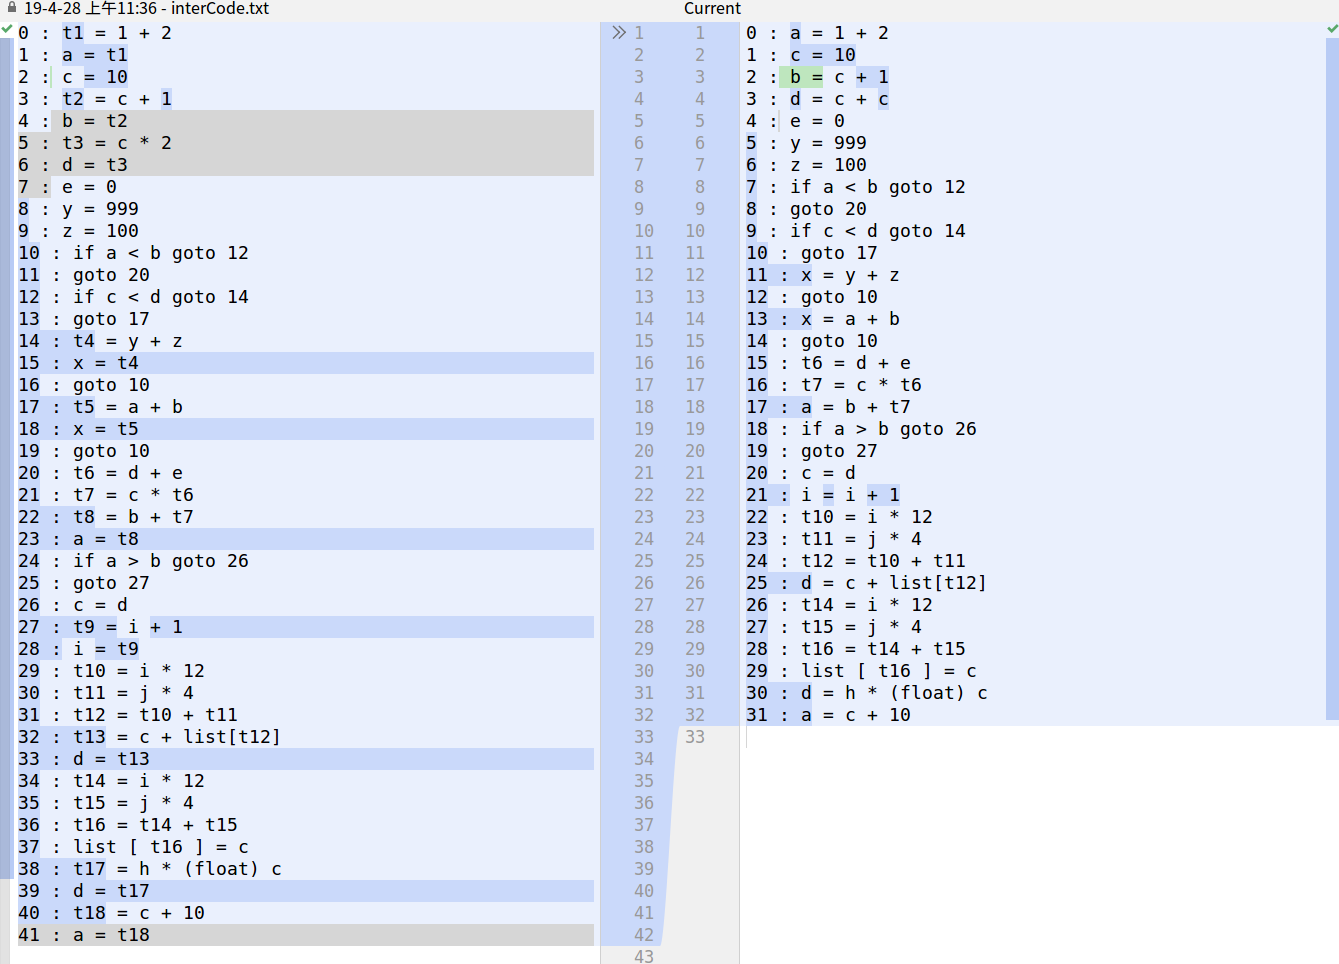
\includegraphics[width=1\linewidth]{media/contract.png}
    \caption{中间代码优化前后对比}\label{fig:contract}
\end{figure}

\appendix

\section{源代码}
\begin{itemize}
    \item \texttt{src/css/}内包含GUI使用的css文件。
    \item \texttt{src/lexer/}内包含词法分析部分使用到的源码。
    \item \texttt{src/parser/}内包含了语法和语义分析部分使用到的源码。
    \item \texttt{src/symbols/}内包含了符号表部分的源码。
    \item \texttt{Main.java}为GUI形式的Compiler主函数,\texttt{sample.fxml}为\texttt{JavaFX}的配置文件。
\end{itemize}
\section{GUI展示}
\begin{figure}[H]
    \centering
    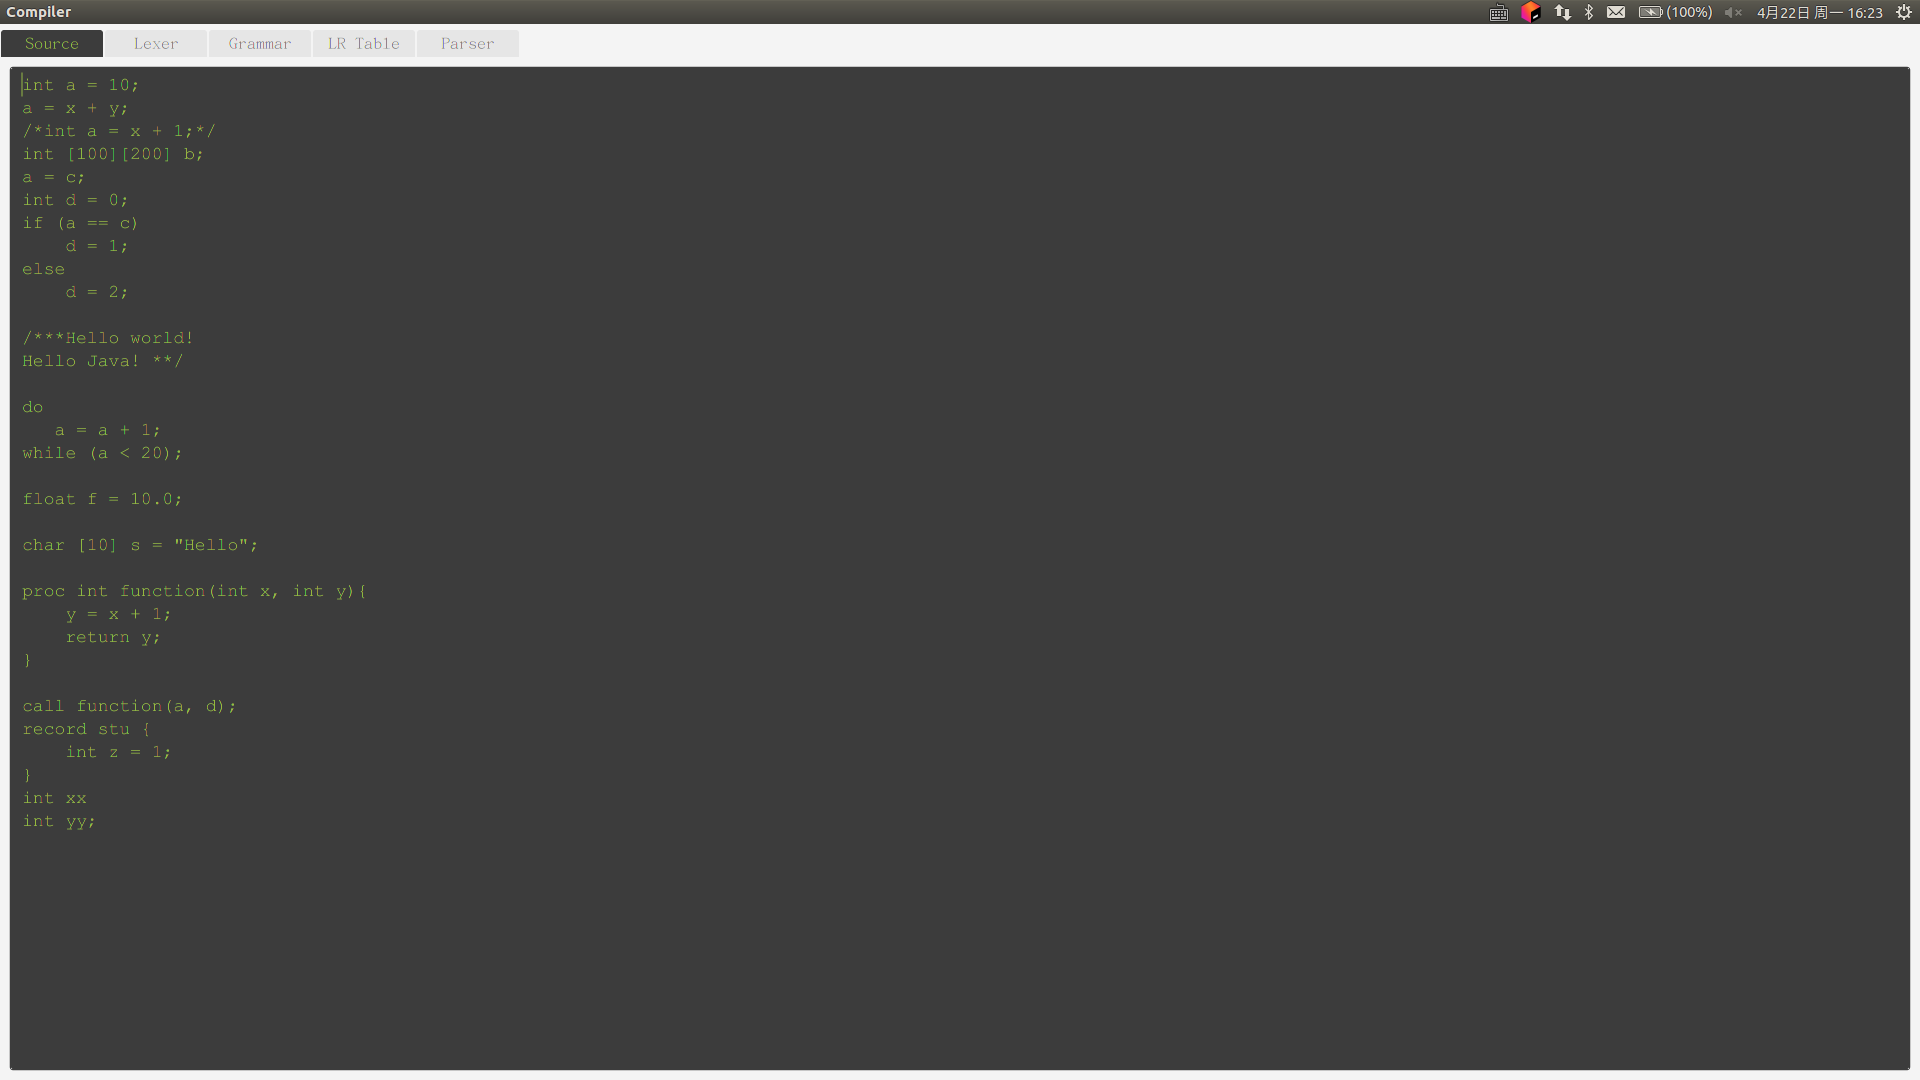
\includegraphics[width=1\linewidth]{media/compiler-source.png}
    \caption{源码部分}
\end{figure}
\begin{figure}[H]
    \centering
    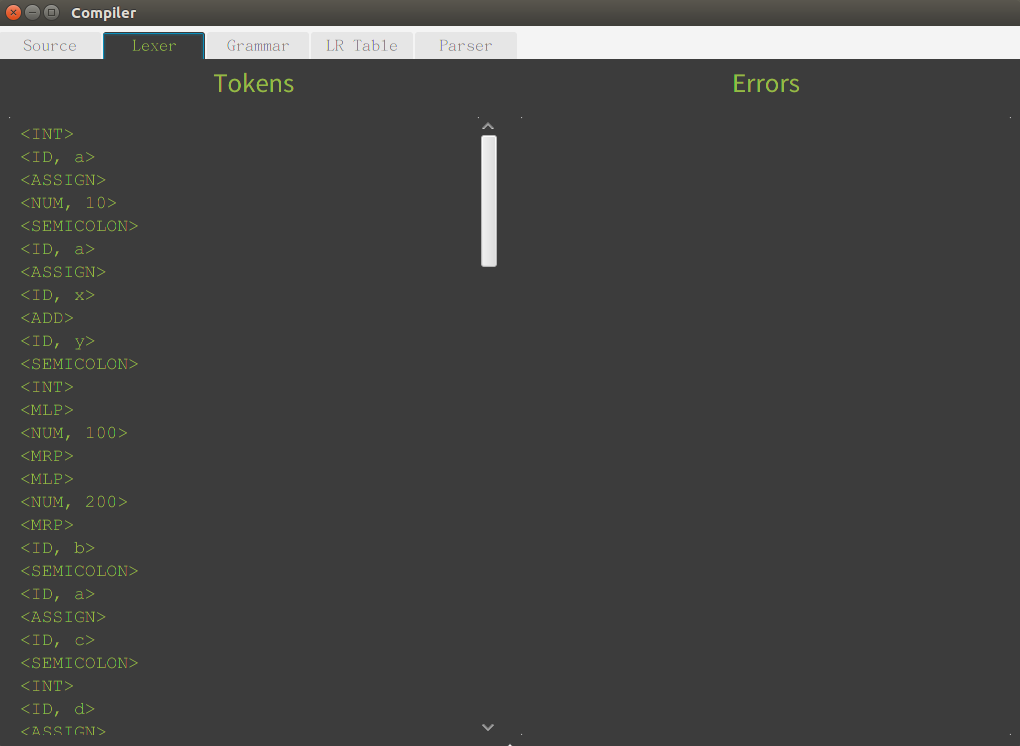
\includegraphics[width=1\linewidth]{media/compiler-lexer.png}
    \caption{Lexer部分}
\end{figure}
\begin{figure}[H]
    \centering
    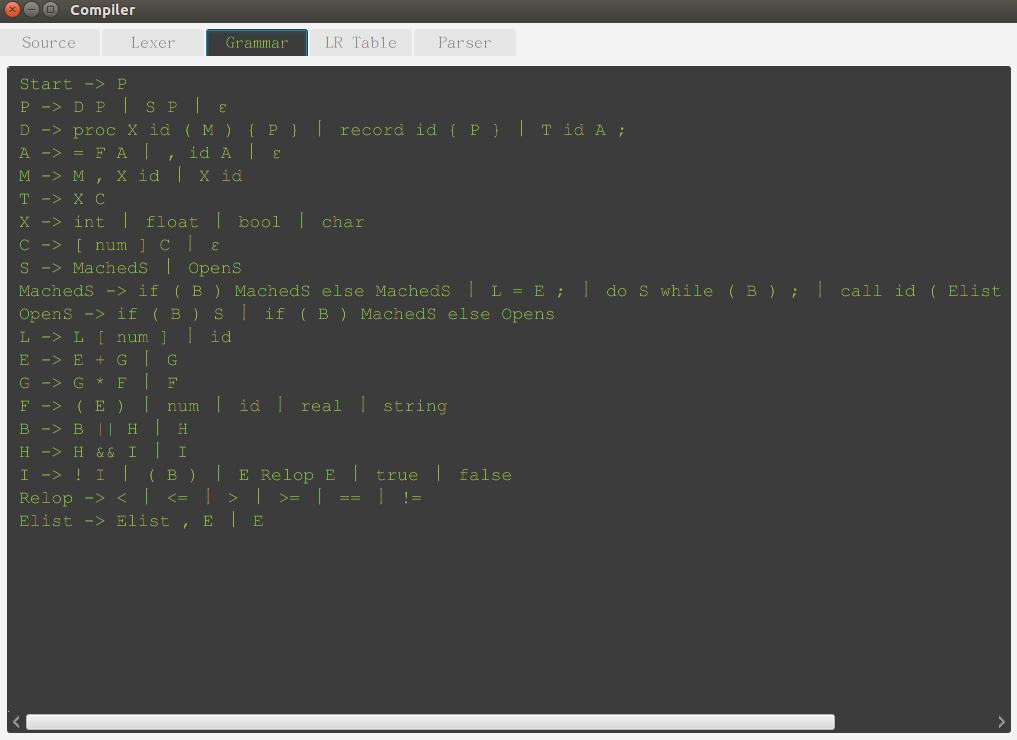
\includegraphics[width=1\linewidth]{media/compiler-grammar.png}
    \caption{文法部分}
\end{figure}
\begin{figure}[H]
    \centering
    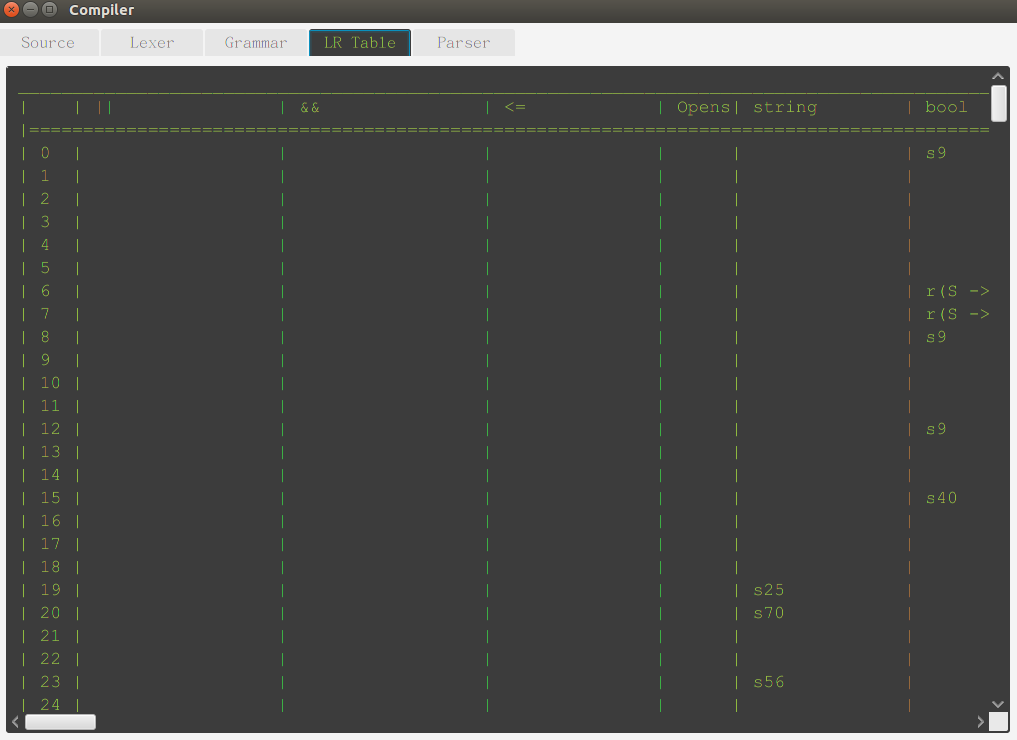
\includegraphics[width=1\linewidth]{media/compiler-lrTable.png}
    \caption{LR分析表部分}
\end{figure}
\begin{figure}[H]
    \centering
    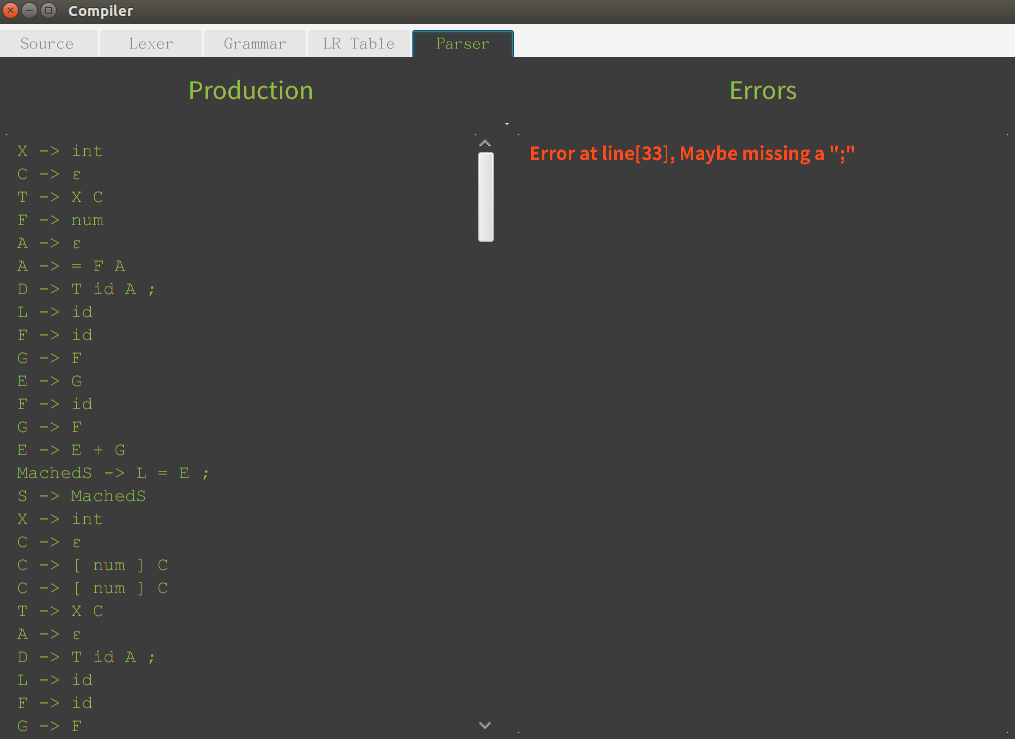
\includegraphics[width=1\linewidth]{media/compiler-parser.png}
    \caption{Parser部分}
\end{figure}
\begin{figure}[H]
    \centering
    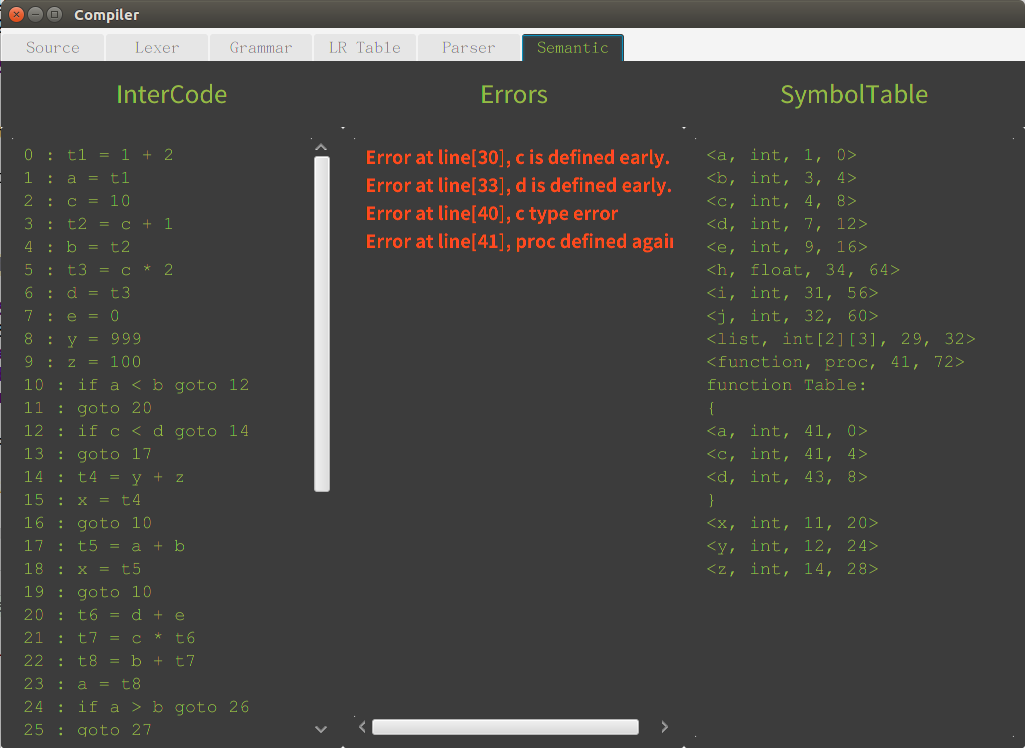
\includegraphics[width=1\linewidth]{media/semantic_compiler.png}
    \caption{语义分析部分}
\end{figure}
\section{参考文献}
\begin{thebibliography}{20}
    \bibitem{dragon-book} Aho A V, Sethi R, Ullman J D. Compilers, principles, techniques[J]. Addison wesley, 1986, 7(8): 9.
\end{thebibliography}

\end{document}
